\subsection{Own Vision Algorithm}
\label{subsec:our_vision}
In Section \ref{subsec:lit_vision}, a number of the vision-based navigation methods used in literatures were briefly introduced and discussed. Although these methods have shown considerably good results in certain work domains, our team decided to come up with more simple method for the obstacle detection and avoidance. The rationale behind this is as follows:
\begin{itemize}
	\item Lucas-Kanade optic flow generation from Harris corner detector or FAST feature detector will not work well unless the obstacles have many "features" on their surface. In the competition, monotonic orange poles and a black wall will be used, and hence we anticipate that there will not be many features available on the texture of the obstacles.
	\item For the same reason, it will be very difficult to compute the Time-to-Contact because it primarily uses the optical flow vectors.
	\item Object recognition or image classification  method can be difficult for tuning and other practical reasons. For example, in order to avoid the orange poles, one cannot simply judge from the overall color of the image as to whether the obstacle is close enough or not. This is because there are cases where multiple poles are visible in the image, although none of them are close enough to the drone. Also, the poles appearing from the "blind spot" of the camera's view are more likely to be hit than the poles located straight ahead (These are verified during the tests). In comparison to other simpler methods, the object recognition will not allow for a flexible adaption to account for all these various situations.
	\item As the drone has only one front camera, the mapping techniques, such as SLAM, will take considerably more computational time and memory. This technique does not go along well with the objective of the competition which is to enable the drone travel as much as possible while minimizing the collisions.
\end{itemize}

For these reasons, it was necessary to come up with much simpler vision algorithm which can be implemented and tested easily. The proposed vision algorithm (Figure \ref{own_vision}) uses a simple color thresholding method for the detection of specified obstacles, which is done in the following steps:
\begin{enumerate}
	\item Take only the bottommost row of the pixels in the image as input. Note that the floor will be visible until the distance between the drone and an obstacle standing on the floor becomes lower than a certain threshold distance, assuming that the drone moves slowly in a hovering flight at a fixed altitude. For the visualization, refer to Section \ref{subsec:lin_sim}.
	\item First of all, the drone should avoid the black wall. By setting a intensity (i.e. Y color channel)  threshold, convert the bottommost pixel row into a binary row which has the elements of value 1 and 0 (i.e. 1 if the pixel intensity value is lower than the threshold, and 0 other wise). Therefore, if the image of the black wall is captured at the bottommost row, it will be indicated by the continuous sequence of 1's.
	\item Count the number of continuous 1's, and if the sequence is longer than a certain threshold, namely the "black wall width-threshold", then mark the position as the position of a black wall. For each mark, give the weight based on the detected width. Determine either to turn left or right, depending on the weighted position of the black wall. 
	\item If there is no black wall detected (i.e. no continuous sequence of 1's exceeding the "black wall width threshold"), evaluate the Cr chroma value to detect the orange poles. Generate a binary row in the similar manner as for the black wall detection by setting an appropriate Cr threshold. 
	\item In order to react more quickly and sensitively towards the poles appearing from the sideways, evaluate the left- and right-end of the Cr binary row to see if there is any shorter continuous sequence of 1's appearing from the sides. This necessitates a different type of width-threshold on the sides, namely the "orange pole sideway threshold". If there is no detection of an orange pole on the sides, continue to the next step.
	\item Using the analogous procedure as for the black wall detection, determine either to turn left or right, depending on the weighted position of the orange pole which can be computed using another width-threshold, namely the "orange pole width-threshold".
	\item If there is still no detection of the continuous sequence of 1 which exceeds any of the above-mentioned width-thresholds, then yield a command to fly forward.
\end{enumerate}

\begin{figure}[h]
	\centering
	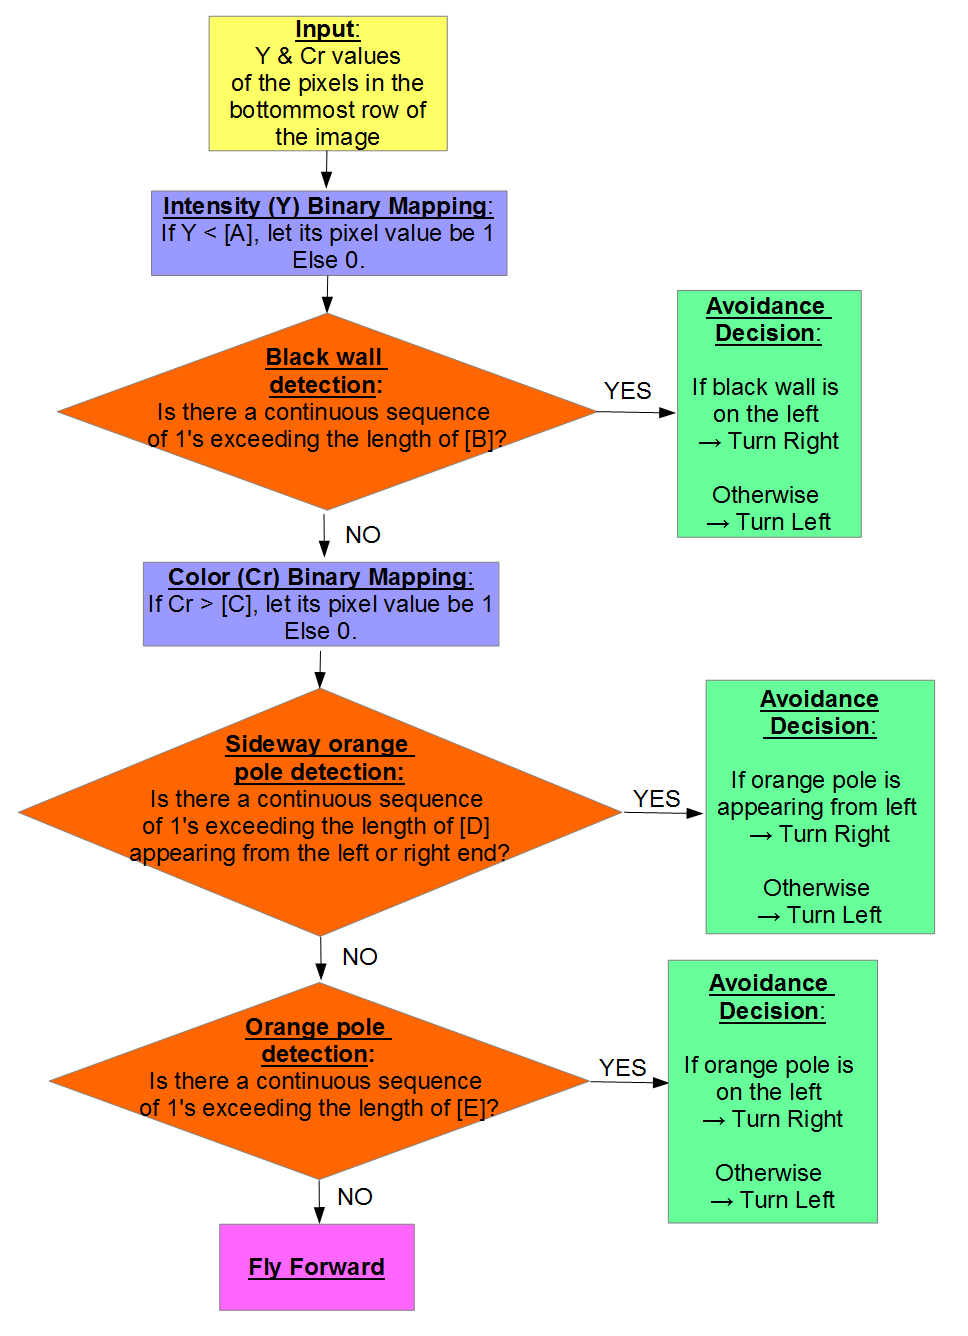
\includegraphics[width = 0.5\textwidth]{Figures/vision.png}
	\caption{Own Vision algorithm for obstacle detection and avoidance. A to E represent various threshold values}
	\label{own_vision}
\end{figure}

The proposed vision algorithm has the following advantages: first of all, there are many tuning parameters (e.g. color-thresholds and width-thresholds). This means that it is possible to adjust the system by trial and error in a flexible manner. For example, the color-thresholds can be easily varied and/or combined to detect specific colors of the obstacle, or the width-thresholds can be changed to adjust the stopping distance from the detected obstacle. Also, it is possible to test the vision algorithm with static images. This allows the tuning easier as the drone does not necessarily have to move around to detect the obstacles. Moreover, the fact that only the bottommost pixel rows are evaluated makes the computation extremely fast; only 640 pixels are accessed. Last but not least, the algorithm has a practical strength as the code is relatively short and simple, which allows for an easy implementation, variation, and debugging.\\

The proposed vision algorithm has the following limitations: first, the collision performance of the drone is largely dependent on the tuning of the parameters due to the high sensitivity. The tuning procedure is thus usually very time-consuming. Also, the drone cannot fly too fast because (1) it should be able to stop well ahead of the obstacle, thereby ensuring a sufficient stopping distance, and (2) it should maintain the bank angle small in order to keep the front camera pointing horizontally forward for the detection of the obstacles ahead. Furthermore, since the proposed vision algorithm yields the control command entirely based on the individual image captured at each frame, it is subject to erroneous obstacle detection caused by the motion blur. Last of all, the biggest limitation of the algorithm would be that it can only work in the Cyberzoo environment with orange poles and black walls as obstacles, and the monochromatic floor and background which have different colors than the obstacles. The algorithm can easily fail if, for example, the floor was painted in a orange or completely black color.